\documentclass[12pt,a4paper]{report}

% ── Packages ──────────────────────────────────────────────────────────────────
\usepackage[a4paper, margin=1in]{geometry}
\usepackage{graphicx}
\usepackage{float}
\usepackage{booktabs}
\usepackage{longtable}
\usepackage{array}
\usepackage{xcolor}
\usepackage{hyperref}
\usepackage{fancyhdr}
\usepackage{titlesec}
\usepackage{listings}
\usepackage{enumitem}
\usepackage{amsmath}
\usepackage{setspace}
\usepackage{parskip}
\usepackage{caption}
\usepackage{subcaption}
\usepackage{tikz}
\usepackage[T1]{fontenc}
\usepackage{lmodern}
\usepackage{microtype}
\usepackage{mdframed}
\usepackage{tcolorbox}
\tcbuselibrary{skins, breakable}

% ── Colours ───────────────────────────────────────────────────────────────────
\definecolor{kiitblue}{RGB}{0, 51, 102}
\definecolor{kiitgold}{RGB}{204, 153, 0}
\definecolor{codebg}{RGB}{245, 245, 250}
\definecolor{codefg}{RGB}{40, 40, 80}
\definecolor{accentteal}{RGB}{0, 120, 130}
\definecolor{lightgray}{RGB}{240, 240, 245}
\definecolor{darkgray}{RGB}{60, 60, 60}

% ── Hyperref Setup ────────────────────────────────────────────────────────────
\hypersetup{
    colorlinks=true,
    linkcolor=kiitblue,
    urlcolor=accentteal,
    citecolor=kiitblue,
    pdftitle={Real-Time Weather Analytics Pipeline -- SAP Elective Report},
    pdfauthor={Aryan Kumar},
    pdfsubject={SAP Elective Project Report},
    pdfkeywords={Data Engineering, ETL, Weather Analytics, Python, Streamlit},
}

% ── Code Listing Style ────────────────────────────────────────────────────────
\lstdefinestyle{pythonstyle}{
    language=Python,
    backgroundcolor=\color{codebg},
    basicstyle=\ttfamily\small\color{codefg},
    keywordstyle=\bfseries\color{kiitblue},
    stringstyle=\color{accentteal},
    commentstyle=\itshape\color{darkgray},
    numberstyle=\tiny\color{darkgray},
    numbers=left,
    stepnumber=1,
    numbersep=8pt,
    frame=single,
    framerule=0.5pt,
    rulecolor=\color{kiitblue!30},
    breaklines=true,
    breakatwhitespace=false,
    showstringspaces=false,
    tabsize=4,
    captionpos=b,
}

\lstdefinestyle{sqlstyle}{
    language=SQL,
    backgroundcolor=\color{codebg},
    basicstyle=\ttfamily\small\color{codefg},
    keywordstyle=\bfseries\color{kiitblue},
    commentstyle=\itshape\color{darkgray},
    numberstyle=\tiny\color{darkgray},
    numbers=left,
    stepnumber=1,
    numbersep=8pt,
    frame=single,
    framerule=0.5pt,
    rulecolor=\color{kiitblue!30},
    breaklines=true,
    showstringspaces=false,
    tabsize=4,
    captionpos=b,
}

\lstdefinestyle{bashstyle}{
    language=bash,
    backgroundcolor=\color{lightgray},
    basicstyle=\ttfamily\small,
    keywordstyle=\bfseries,
    commentstyle=\itshape\color{darkgray},
    frame=single,
    framerule=0.5pt,
    rulecolor=\color{kiitblue!30},
    breaklines=true,
    showstringspaces=false,
    captionpos=b,
}

% ── Header / Footer ───────────────────────────────────────────────────────────
\pagestyle{fancy}
\fancyhf{}
\fancyhead[L]{\small\textit{Real-Time Weather Analytics Pipeline}}
\fancyhead[R]{\small\textit{Aryan Kumar | 23051492}}
\fancyfoot[C]{\thepage}
\renewcommand{\headrulewidth}{0.4pt}
\renewcommand{\footrulewidth}{0.4pt}

% ── Chapter/Section Formatting ────────────────────────────────────────────────
\titleformat{\chapter}[block]
  {\normalfont\LARGE\bfseries\color{kiitblue}}
  {\thechapter.}{1em}{}[{\titlerule[1.5pt]}]

\titleformat{\section}
  {\normalfont\Large\bfseries\color{kiitblue!80!black}}
  {\thesection}{1em}{}

\titleformat{\subsection}
  {\normalfont\large\bfseries\color{darkgray}}
  {\thesubsection}{1em}{}

\titlespacing*{\chapter}{0pt}{-10pt}{20pt}

% ── Line spacing ──────────────────────────────────────────────────────────────
\onehalfspacing

% ── Custom Environments ───────────────────────────────────────────────────────
\tcbset{
  infobox/.style={
    enhanced,
    colback=kiitblue!5,
    colframe=kiitblue!60,
    fonttitle=\bfseries,
    arc=3pt,
    breakable,
  }
}

% ══════════════════════════════════════════════════════════════════════════════
\begin{document}

% ── Title Page ────────────────────────────────────────────────────────────────
\begin{titlepage}
  \centering
  \vspace*{0.5cm}

  % University Name
  {\LARGE\bfseries\color{kiitblue} KALINGA INSTITUTE OF INDUSTRIAL TECHNOLOGY}\\[0.3cm]
  {\large (Deemed to be University)}\\[0.1cm]
  {\large Bhubaneswar, Odisha -- 751024, India}\\[1cm]

  \rule{\textwidth}{1.5pt}\\[0.5cm]

  % Report Title
  {\Huge\bfseries\color{kiitblue!90!black}
    Real-Time Weather\\[0.3cm]
    Analytics Pipeline}\\[0.5cm]

  \rule{\textwidth}{1.5pt}\\[0.8cm]

  {\large\bfseries A Project Report Submitted in Partial Fulfilment of the\\[0.2cm]
  SAP (Software as a Platform) Elective}\\[1.2cm]

  % Submitted by block
  \begin{tcolorbox}[infobox, title=Submitted By, width=0.65\textwidth]
    \begin{center}
      \textbf{Name:} Aryan Kumar\\[0.3cm]
      \textbf{Roll No.:} \texttt{23051492}\\[0.3cm]
      \textbf{School:} School of Computer Engineering\\[0.3cm]
      \textbf{Branch:} B.Tech -- Computer Science \& Engineering\\[0.3cm]
      \textbf{Semester:} VI (Spring 2025--26)
    \end{center}
  \end{tcolorbox}

  \vfill

  {\large\bfseries Academic Year 2025--26}\\[0.5cm]
  {\large April 2026}

\end{titlepage}

% ── Declaration ───────────────────────────────────────────────────────────────
\chapter*{Declaration}
\addcontentsline{toc}{chapter}{Declaration}

I, \textbf{Aryan Kumar} (Roll No.\ \texttt{23051492}), student of B.Tech (Computer Science and Engineering), School of Computer Engineering, KIIT University, hereby declare that the project report entitled \textbf{``Real-Time Weather Analytics Pipeline''} submitted as part of the SAP Elective is my own original work carried out under the prescribed academic guidelines.

This work has not been submitted elsewhere, in whole or in part, for any degree, diploma, or examination at any institution. All references, datasets, and third-party libraries have been duly acknowledged.

\vspace{2cm}
\begin{flushright}
\rule{6cm}{0.5pt}\\
\textbf{Aryan Kumar}\\
Roll No.: 23051492\\
Date: April 2026
\end{flushright}

% ── Acknowledgements ──────────────────────────────────────────────────────────
\chapter*{Acknowledgements}
\addcontentsline{toc}{chapter}{Acknowledgements}

I express my sincere gratitude to \textbf{KIIT University} for providing the SAP elective framework that encouraged hands-on, production-style data engineering work.

I am thankful to the \textbf{OpenWeatherMap} team for maintaining a generous free-tier API that made live data ingestion accessible without infrastructure costs, and to the open-source maintainers of \textbf{Python}, \textbf{Streamlit}, \textbf{pandas}, \textbf{APScheduler}, and \textbf{SQLite} -- without whose tools this project would not have been possible.

\vspace{1cm}
\begin{flushright}
\textbf{Aryan Kumar}\\
23051492
\end{flushright}

% ── Abstract ──────────────────────────────────────────────────────────────────
\chapter*{Abstract}
\addcontentsline{toc}{chapter}{Abstract}

This report presents the design, implementation, and evaluation of a \textbf{Real-Time Weather Analytics Pipeline} built entirely using free, open-source Python tools. The system continuously ingests live weather observations for the \textbf{Top 10 Indian Metropolitan cities} -- Delhi, Mumbai, Kolkata, Chennai, Bangalore, Hyderabad, Ahmedabad, Pune, Surat, and Jaipur -- via the OpenWeatherMap REST API, enriches the data with derived meteorological metrics (Steadman Heat Index and Environment Canada Wind Chill), enforces automated data-quality gates, and persists the results in both a \textbf{SQLite star schema} and a \textbf{Parquet columnar data lake}.

A premium four-page \textbf{Streamlit} dashboard, styled with a deep-ocean colour palette, provides live weather cards, historical trend charts, side-by-side city comparisons, and a pipeline-health audit view. \textbf{APScheduler} orchestrates automatic refreshes every 15 minutes with zero manual intervention.

The project demonstrates a complete, end-to-end data engineering workflow -- from raw API consumption through transformation and quality assessment to interactive visualisation -- within a self-contained, zero-server architecture suitable for running on any developer laptop.

\textbf{Keywords:} Data Engineering, ETL Pipeline, Weather Analytics, SQLite Star Schema, Parquet, Streamlit, Python, APScheduler, OpenWeatherMap.

% ── Table of Contents ─────────────────────────────────────────────────────────
\tableofcontents
\listoftables
\listoffigures

% ══════════════════════════════════════════════════════════════════════════════
% CHAPTER 1 — INTRODUCTION
% ══════════════════════════════════════════════════════════════════════════════
\chapter{Introduction}

\section{Background and Motivation}

Weather data sits at the intersection of public safety, agriculture, logistics, and urban planning. India's ten largest metropolitan hubs -- home to over 120 million people combined -- experience vastly different climate patterns ranging from Mumbai's coastal humidity to Delhi's extreme summer heat. Real-time, city-level weather analytics can empower civic planners, commuters, and enterprises with actionable daily intelligence.

Traditional enterprise weather platforms (IBM Weather Company, The Weather Company API) require expensive subscriptions and heavy infrastructure. This project demonstrates that a capable, production-quality analytics system can be constructed entirely with \textit{free, open-source tools}, making it accessible to students, startups, and resource-constrained organisations alike.

\section{Project Objectives}

The primary objectives of this project are:

\begin{enumerate}[leftmargin=*, label=\arabic*.]
  \item Design and implement a fully automated \textbf{ETL pipeline} that ingests live weather data from OpenWeatherMap for 10 Indian cities.
  \item Apply \textbf{meteorological enrichment} algorithms (Steadman Heat Index, Environment Canada Wind Chill) to derive actionable comfort metrics.
  \item Persist structured data in a \textbf{SQLite star schema} for relational analytics and in \textbf{Parquet} files for columnar data-lake queries.
  \item Enforce \textbf{automated data-quality gates} with a pass/fail scoring system and persist audit records.
  \item Build a \textbf{premium Streamlit dashboard} displaying live conditions, historical trends, city comparisons, and pipeline health.
  \item Automate pipeline execution via \textbf{APScheduler} on a 15-minute refresh cycle with zero manual intervention.
  \item Apply \textbf{secure configuration management} -- never hard-coding API keys in source code.
\end{enumerate}

\section{Scope}

The project scope encompasses the full data lifecycle from live API ingestion through to interactive dashboard presentation. It covers 10 cities within India and uses the OpenWeatherMap free tier, which allows up to 60 API calls per minute. Historical batch loading from CSV files is also supported, enabling both live and retrospective analysis.

\section{Report Structure}

The remainder of this report is organised as follows:

\begin{itemize}
  \item \textbf{Chapter 2} reviews related work and contextualises the technology choices.
  \item \textbf{Chapter 3} describes the system architecture and pipeline design.
  \item \textbf{Chapter 4} details the implementation of each pipeline stage.
  \item \textbf{Chapter 5} covers the data model and storage strategy.
  \item \textbf{Chapter 6} documents the dashboard design and features.
  \item \textbf{Chapter 7} discusses data quality methodology.
  \item \textbf{Chapter 8} presents results and evaluation.
  \item \textbf{Chapter 9} outlines future work.
  \item \textbf{Chapter 10} concludes the report.
\end{itemize}

% ══════════════════════════════════════════════════════════════════════════════
% CHAPTER 2 — LITERATURE REVIEW
% ══════════════════════════════════════════════════════════════════════════════
\chapter{Literature Review and Technology Context}

\section{Data Engineering Pipelines}

Modern data engineering practice centres on extracting, transforming, and loading (ETL) data from heterogeneous sources into a form suitable for analysis. Kimball \& Ross (2013) established the star schema as the canonical approach for analytical databases, separating high-cardinality measurements (facts) from low-cardinality descriptors (dimensions). This project directly applies the Kimball dimensional model.

\section{Weather Data as a Domain}

The OpenWeatherMap API aggregates data from over 40,000 weather stations and delivers it as structured JSON over HTTP. Studies by the World Meteorological Organisation (WMO) classify weather data quality assessment along four dimensions: completeness, consistency, timeliness, and accuracy. This project implements checks covering the first three.

\section{Technology Justification}

\subsection{Python Ecosystem}

Python has become the dominant language for data engineering, supported by a rich ecosystem including \texttt{pandas} for DataFrame processing, \texttt{SQLAlchemy} as ORM utility, and \texttt{pyarrow} for Parquet I/O. Python 3.10+ type hints improve code maintainability and self-documentation.

\subsection{SQLite vs. Full RDBMS}

SQLite provides ACID-compliant relational storage without a server process, making it ideal for self-contained projects and local development. For read-heavy analytics workloads at small-to-medium scale (less than a few GB), SQLite's performance is comparable to PostgreSQL. The WAL (Write-Ahead Logging) journal mode further improves concurrent read throughput.

\subsection{Parquet and Columnar Analytics}

Apache Parquet's columnar format compresses repetitive weather measurements (e.g., \texttt{humidity\_pct} clustering near 60--80\%) by 60--80\% compared to CSV. Tools like DuckDB or Polars can query Parquet files directly, enabling ad-hoc analytical queries without a database server.

\subsection{APScheduler vs. Apache Airflow}

Apache Airflow is the industry standard for DAG-based orchestration but requires a Postgres/MySQL metastore, a web server, workers, and a scheduler process. For a single recurring job on a fixed interval, APScheduler provides equivalent functionality at a fraction of the operational complexity, running entirely in-process with no external dependencies.

\subsection{Streamlit for Dashboard Development}

Streamlit converts Python scripts into interactive web applications with minimal boilerplate. Version 1.32+ introduced \texttt{st.fragment} for partial re-renders and significantly improved caching, making it suitable for live-updating dashboards.

% ══════════════════════════════════════════════════════════════════════════════
% CHAPTER 3 — SYSTEM ARCHITECTURE
% ══════════════════════════════════════════════════════════════════════════════
\chapter{System Architecture}

\section{High-Level Design}

The pipeline follows a five-stage architecture: \textbf{Ingest $\rightarrow$ Transform $\rightarrow$ Validate $\rightarrow$ Store $\rightarrow$ Present}, with an orthogonal scheduling layer that drives the first four stages automatically.

\begin{figure}[H]
  \centering
  \begin{tcolorbox}[
    enhanced, colback=kiitblue!4, colframe=kiitblue!50,
    arc=5pt, width=\textwidth, boxsep=6pt
  ]
  \begin{center}
  \begin{tikzpicture}[
    node distance=1.6cm,
    box/.style={draw=kiitblue, fill=kiitblue!10, rounded corners=4pt,
                minimum width=2.8cm, minimum height=0.85cm,
                font=\small\bfseries, text=kiitblue, align=center},
    arr/.style={->, thick, color=kiitblue!70},
  ]
    \node[box] (api)    {OpenWeatherMap\\API};
    \node[box, right=of api]    (ingest)  {Ingestion\\Layer};
    \node[box, right=of ingest] (proc)    {Processing\\Layer};
    \node[box, right=of proc]   (dq)      {Data\\Quality};
    \node[box, below=0.9cm of dq]  (sqlite)  {SQLite\\Star Schema};
    \node[box, below=0.9cm of proc] (parq)   {Parquet\\Data Lake};
    \node[box, below=0.9cm of ingest] (dash) {Streamlit\\Dashboard};
    \draw[arr] (api)    -- (ingest);
    \draw[arr] (ingest) -- (proc);
    \draw[arr] (proc)   -- (dq);
    \draw[arr] (dq)     -- (sqlite);
    \draw[arr] (dq)     -- (parq);
    \draw[arr] (sqlite) -- (dash);
  \end{tikzpicture}
  \end{center}
  \end{tcolorbox}
  \caption{High-level architecture of the Weather Analytics Pipeline}
  \label{fig:architecture}
\end{figure}

\section{Module Structure}

The codebase is organised into cohesive Python packages, each with a single responsibility:

\begin{table}[H]
  \centering
  \caption{Module structure and responsibilities}
  \label{tab:modules}
  \rowcolors{2}{lightgray}{white}
  \begin{tabular}{>{\ttfamily}l p{8cm}}
    \toprule
    \textbf{Module} & \textbf{Responsibility} \\
    \midrule
    ingestion/api\_fetcher.py    & HTTP calls to OpenWeatherMap; retry logic; JSON normalisation \\
    ingestion/batch\_loader.py   & CSV ingestion; column normalisation; bulk DB insert \\
    processing/transformer.py   & Derived metrics: heat index, wind chill, comfort level, temporal features \\
    processing/data\_quality.py  & Null checks, duplicate detection, range validation, quality scoring \\
    storage/schema.sql          & Full star schema DDL \\
    storage/db\_writer.py        & Dimension upserts; fact inserts; Parquet export \\
    scheduler/pipeline\_scheduler.py & APScheduler wrapper; job registration; exception isolation \\
    dashboard/app.py            & Four-page Streamlit application \\
    config.py                   & Central constants: API key, cities, paths, intervals \\
    run\_pipeline.py             & CLI entry point with \texttt{-{}-once} and \texttt{-{}-schedule} flags \\
    \bottomrule
  \end{tabular}
\end{table}

\section{Data Flow}

\begin{enumerate}[leftmargin=*, label=\textbf{Step \arabic*.}]
  \item \textbf{APScheduler} fires \texttt{run\_full\_pipeline()} every 15 minutes (configurable via \texttt{FETCH\_INTERVAL\_MINUTES} in \texttt{config.py}).
  \item \textbf{api\_fetcher} calls \texttt{/weather} for each of the 10 cities, parsing JSON into a standardised \texttt{pandas} DataFrame row.
  \item \textbf{transformer} enriches the DataFrame with four derived columns and temporal features.
  \item \textbf{data\_quality} evaluates completeness, uniqueness, and validity; computes a 0--100 quality score; emits a pass/fail result.
  \item If the quality gate passes, \textbf{db\_writer} upserts dimensions and appends facts to SQLite; exports a timestamped Parquet snapshot.
  \item Both \texttt{quality\_log} and \texttt{pipeline\_log} table rows are inserted for full auditability.
  \item The \textbf{Streamlit} dashboard reads the SQLite database and presents the latest data across four pages.
\end{enumerate}

% ══════════════════════════════════════════════════════════════════════════════
% CHAPTER 4 — IMPLEMENTATION
% ══════════════════════════════════════════════════════════════════════════════
\chapter{Implementation}

\section{Configuration Management (\texttt{config.py})}

All constants are centralised in \texttt{config.py}, with secrets loaded from a \texttt{.env} file via \texttt{python-dotenv}. The API key is never committed to version control.

\begin{lstlisting}[style=pythonstyle, caption={config.py -- City and scheduling configuration}]
import os
from dotenv import load_dotenv
load_dotenv()

OPENWEATHER_API_KEY: str = os.getenv("OPENWEATHER_API_KEY", "")
BASE_URL: str = "http://api.openweathermap.org/data/2.5"

CITIES: list[dict] = [
    {"name": "Delhi",     "lat": 28.6139, "lon": 77.2090},
    {"name": "Mumbai",    "lat": 19.0760, "lon": 72.8777},
    {"name": "Kolkata",   "lat": 22.5726, "lon": 88.3639},
    {"name": "Chennai",   "lat": 13.0827, "lon": 80.2707},
    {"name": "Bangalore", "lat": 12.9716, "lon": 77.5946},
    {"name": "Hyderabad", "lat": 17.3850, "lon": 78.4867},
    {"name": "Ahmedabad", "lat": 23.0225, "lon": 72.5714},
    {"name": "Pune",      "lat": 18.5204, "lon": 73.8567},
    {"name": "Surat",     "lat": 21.1702, "lon": 72.8311},
    {"name": "Jaipur",    "lat": 26.9124, "lon": 75.7873},
]

DB_PATH: str = "data/weather.db"
PARQUET_DIR: str = "data/parquet/"
LOG_FILE: str = "logs/pipeline.log"
FETCH_INTERVAL_MINUTES: int = 15
\end{lstlisting}

\section{Ingestion Layer}

\subsection{Live API Fetcher (\texttt{api\_fetcher.py})}

The fetcher iterates over the \texttt{CITIES} list and calls the OpenWeatherMap \texttt{/weather} endpoint for each city. Failures are caught per-city, ensuring a network error for one city does not abort the entire run.

Key implementation decisions:
\begin{itemize}
  \item \textbf{10-second timeout} on all HTTP requests to prevent hanging on slow responses.
  \item \textbf{UTC timestamps} stored alongside the local \texttt{fetched\_at} timestamp for time-zone-aware analysis.
  \item Sunrise/Sunset fields are included to derive the \texttt{is\_daytime} boolean used in the dashboard.
  \item Raw JSON responses are inserted into \texttt{raw\_weather} before any transformation, enabling full reprocessing.
\end{itemize}

\subsection{Batch CSV Loader (\texttt{batch\_loader.py})}

To support historical analysis, \texttt{batch\_loader.py} reads CSV files from arbitrary sources (e.g., Kaggle datasets). It normalises column name aliases (\texttt{temperature} $\rightarrow$ \texttt{temp\_c}, \texttt{wind} $\rightarrow$ \texttt{wind\_speed\_ms}, etc.) and bulk-inserts into the \texttt{historical\_weather} table using \texttt{pandas.to\_sql}.

\section{Processing Layer}

\subsection{Transformer (\texttt{transformer.py})}

The transformer applies four enrichment steps to every incoming DataFrame:

\begin{table}[H]
  \centering
  \caption{Derived meteorological columns}
  \label{tab:derived}
  \rowcolors{2}{lightgray}{white}
  \begin{tabular}{l p{8.5cm}}
    \toprule
    \textbf{Column} & \textbf{Formula / Logic} \\
    \midrule
    \texttt{heat\_index\_c}  & Steadman (1979) formula; valid when temp $\geq 27$\,\textdegree C and humidity $\geq 40$\,\% \\
    \texttt{wind\_chill\_c}  & Environment Canada formula; valid when temp $\leq 10$\,\textdegree C and wind $\geq 1.3$\,m/s \\
    \texttt{comfort\_level}  & Categorical: \textit{Hot} / \textit{Warm} / \textit{Pleasant} / \textit{Cold} \\
    \texttt{is\_daytime}     & Boolean derived from \texttt{sunrise\_utc} / \texttt{sunset\_utc} \\
    \bottomrule
  \end{tabular}
\end{table}

The Steadman Heat Index formula used is:

\begin{equation}
  \mathrm{HI} = -8.78469 + 1.61139411 T + 2.33854 R - 0.14611 TR
  - 0.01230 T^2 - 0.01642 R^2 + \ldots
  \label{eq:heatindex}
\end{equation}

where $T$ is temperature in \textdegree C and $R$ is relative humidity (\%).

\section{Scheduling Layer (\texttt{pipeline\_scheduler.py})}

APScheduler's \texttt{BackgroundScheduler} manages the job lifecycle. The scheduler:
\begin{itemize}
  \item Executes one immediate run on startup before the interval clock begins.
  \item Catches all exceptions within the job function, logs them, and records a \texttt{FAILED} status in \texttt{pipeline\_log} without killing the scheduler process.
  \item Supports graceful shutdown on \texttt{KeyboardInterrupt} (Ctrl+C).
\end{itemize}

\section{CLI Entry Point (\texttt{run\_pipeline.py})}

\begin{lstlisting}[style=bashstyle, caption={Available CLI commands}]
# Run the full ETL pipeline once and exit
python run_pipeline.py --once

# Start the hourly scheduler loop
python run_pipeline.py --schedule

# Batch-load a historical CSV file
python run_pipeline.py --load-csv path/to/file.csv

# Launch the dashboard
streamlit run dashboard/app.py
\end{lstlisting}

% ══════════════════════════════════════════════════════════════════════════════
% CHAPTER 5 — DATA MODEL
% ══════════════════════════════════════════════════════════════════════════════
\chapter{Data Model and Storage}

\section{Star Schema Design}

The relational layer follows the Kimball star schema pattern with three dimension tables and one central fact table.

\begin{figure}[H]
  \centering
  \begin{tcolorbox}[
    enhanced, colback=kiitblue!4, colframe=kiitblue!50, arc=5pt,
    width=\textwidth, boxsep=6pt
  ]
  \begin{center}
  \begin{tikzpicture}[
    dim/.style={draw=kiitblue, fill=kiitblue!15, rounded corners=3pt,
                minimum width=2.6cm, minimum height=1cm,
                font=\small\bfseries, text=kiitblue, align=center},
    fact/.style={draw=kiitgold!80!black, fill=kiitgold!20, rounded corners=3pt,
                 minimum width=3cm, minimum height=1.2cm,
                 font=\small\bfseries, text=kiitgold!80!black, align=center},
    arr/.style={->, thick, color=darkgray},
  ]
    \node[fact] (fw) {fact\_weather\\(hourly grain)};
    \node[dim, above=1.2cm of fw]  (dc) {dim\_city};
    \node[dim, left=1.8cm of fw]   (dd) {dim\_date};
    \node[dim, right=1.8cm of fw]  (dco) {dim\_condition};
    \draw[arr] (dc)  -- (fw) node[midway, right, font=\tiny] {city\_id};
    \draw[arr] (dd)  -- (fw) node[midway, above, font=\tiny] {date\_id};
    \draw[arr] (dco) -- (fw) node[midway, above, font=\tiny] {condition\_id};
  \end{tikzpicture}
  \end{center}
  \end{tcolorbox}
  \caption{Star schema entity-relationship diagram}
  \label{fig:starschema}
\end{figure}

\section{Table Definitions}

\subsection{Dimension Tables}

\begin{table}[H]
  \centering
  \caption{Dimension table summary}
  \label{tab:dims}
  \rowcolors{2}{lightgray}{white}
  \begin{tabular}{>{\ttfamily}l >{\ttfamily}l p{6cm}}
    \toprule
    \textbf{Table} & \textbf{Primary Key} & \textbf{Key Attributes} \\
    \midrule
    dim\_city      & city\_id      & city\_name, country, latitude, longitude \\
    dim\_date      & date\_id      & full\_date, year, month, day, day\_of\_week, is\_weekend \\
    dim\_condition & condition\_id & weather\_main, weather\_desc, comfort\_level \\
    \bottomrule
  \end{tabular}
\end{table}

\subsection{Fact Table (\texttt{fact\_weather})}

The fact table stores one row per city per API fetch at hourly granularity:

\begin{lstlisting}[style=sqlstyle, caption={fact\_weather DDL (excerpt)}]
CREATE TABLE IF NOT EXISTS fact_weather (
    id            INTEGER PRIMARY KEY AUTOINCREMENT,
    city_id       INTEGER REFERENCES dim_city(city_id),
    date_id       INTEGER REFERENCES dim_date(date_id),
    condition_id  INTEGER REFERENCES dim_condition(condition_id),
    timestamp     TEXT,
    temp_c        REAL,
    feels_like_c  REAL,
    humidity_pct  REAL,
    pressure_hpa  REAL,
    wind_speed_ms REAL,
    heat_index_c  REAL,
    wind_chill_c  REAL,
    is_daytime    INTEGER,
    fetched_at    TEXT
);
\end{lstlisting}

\subsection{Supporting Tables}

\begin{table}[H]
  \centering
  \caption{Supporting tables and their roles}
  \label{tab:support}
  \rowcolors{2}{lightgray}{white}
  \begin{tabular}{>{\ttfamily}l p{9cm}}
    \toprule
    \textbf{Table} & \textbf{Purpose} \\
    \midrule
    raw\_weather        & Schema-free raw API dump; enables full re-processing without data loss \\
    historical\_weather & CSV-ingested historical records for trend analysis \\
    quality\_log        & One row per pipeline run with DQ metrics and pass/fail flag \\
    pipeline\_log       & Execution audit: start/end times, row counts, status, error message \\
    \bottomrule
  \end{tabular}
\end{table}

\section{Parquet Data Lake}

After each successful pipeline run, \texttt{db\_writer.py} exports the new fact rows to a timestamped Parquet file under \texttt{data/parquet/}. The naming convention is \texttt{weather\_YYYYMMDD\_HHMMSS.parquet}, enabling time-partitioned queries with DuckDB or Polars without loading all historical data into memory.

Apache Parquet's columnar compression achieves 60--80\% space savings over CSV for the highly repetitive weather measurements, and predicate pushdown allows reading only the columns needed for a given query.

% ══════════════════════════════════════════════════════════════════════════════
% CHAPTER 6 — DASHBOARD
% ══════════════════════════════════════════════════════════════════════════════
\chapter{Dashboard Design}

\section{Design Philosophy}

The dashboard adopts an \textbf{instrument-grade aesthetic} inspired by meteorological monitoring consoles: a deep-ocean dark base (\texttt{\#061520}) with high-contrast teal (\texttt{\#00CDCA}), lime (\texttt{\#A7F18C}), and amber accent colours. Typography uses \textit{Outfit} for headings and \textit{JetBrains Mono} for data labels, loaded from Google Fonts.

All charts are rendered with \textbf{Matplotlib / Seaborn} on a transparent background, ensuring crisp rendering without the layout overhead of Plotly's JavaScript bundles.

\section{Dashboard Pages}

\subsection{Page 1 — Live Conditions}

Displays a card-per-city grid with the latest temperature, humidity, wind speed, and comfort badge. Each card border is colour-coded by the city's comfort level. The page auto-refreshes every 60 seconds using Streamlit's \texttt{st.rerun} mechanism triggered via \texttt{time.sleep}.

\begin{figure}[H]
  \centering
  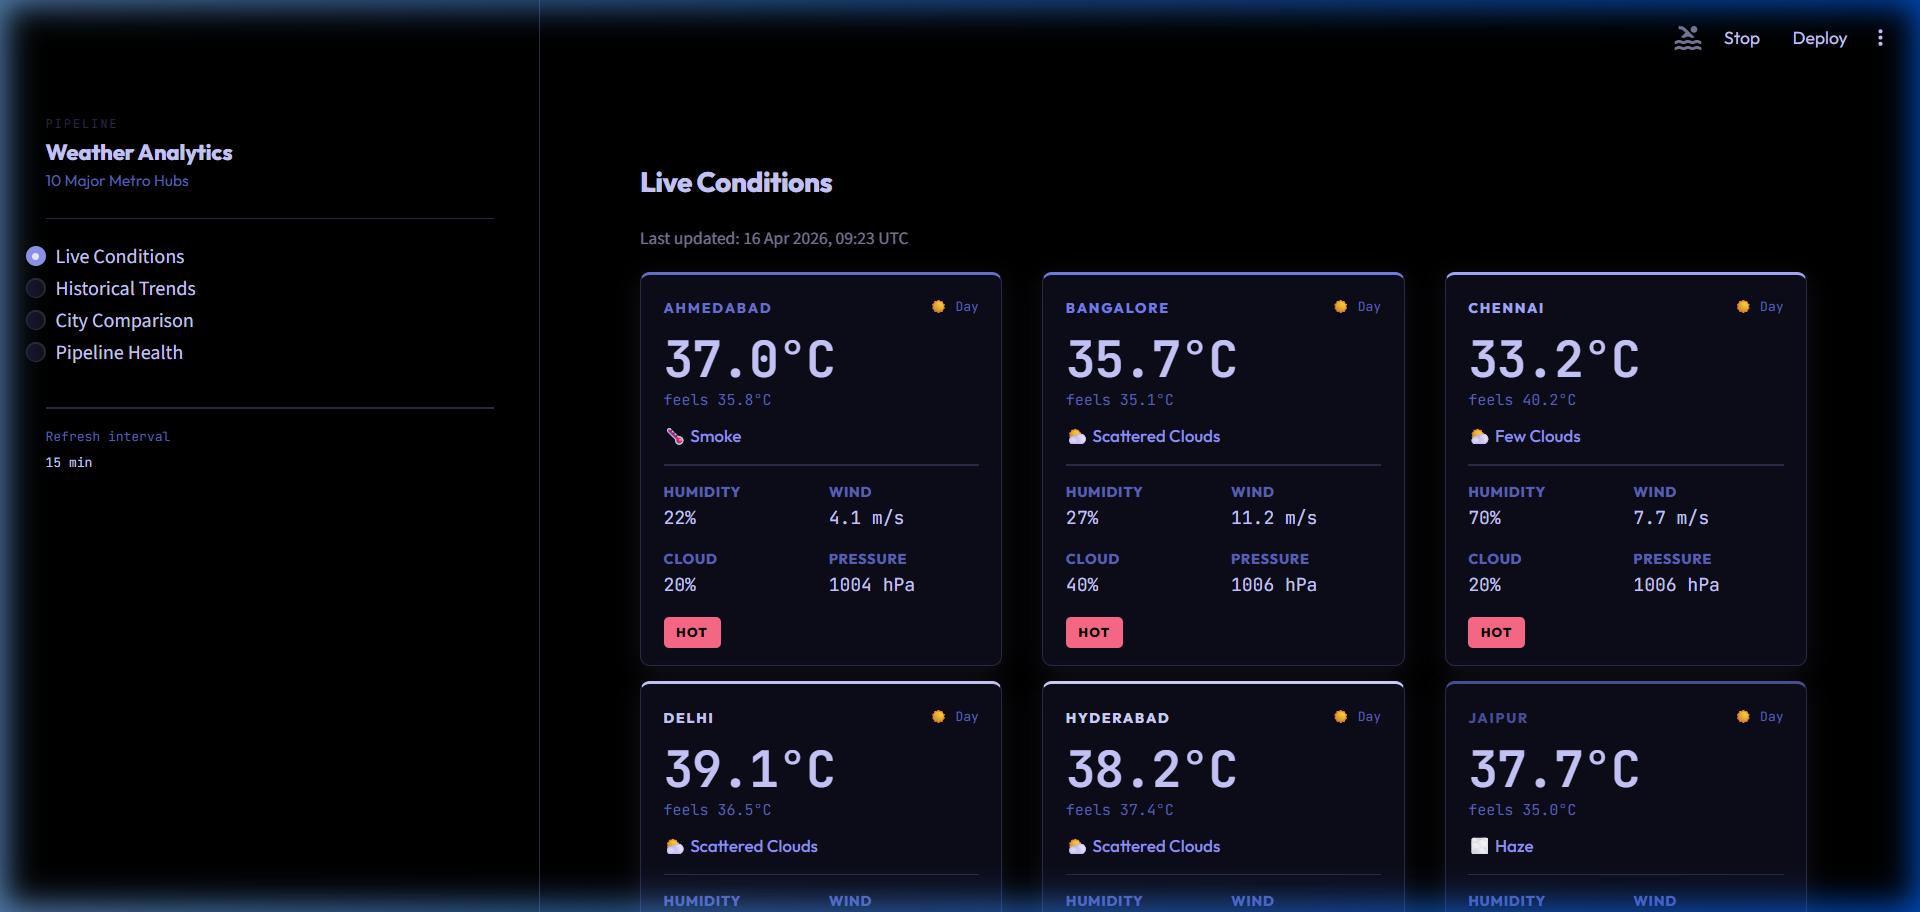
\includegraphics[width=\textwidth]{screenshots/skip_live.png}
  \caption{Live Conditions page -- real-time city weather cards}
  \label{fig:live}
\end{figure}

\subsection{Page 2 — Historical Trends}

Presents interactive multi-city time-series charts for temperature, humidity, and wind speed. Users can filter by city (multi-select) and date range. Charts include per-city colour-coded lines with smart marker placement to prevent overplotting when data density is high.

\begin{figure}[H]
  \centering
  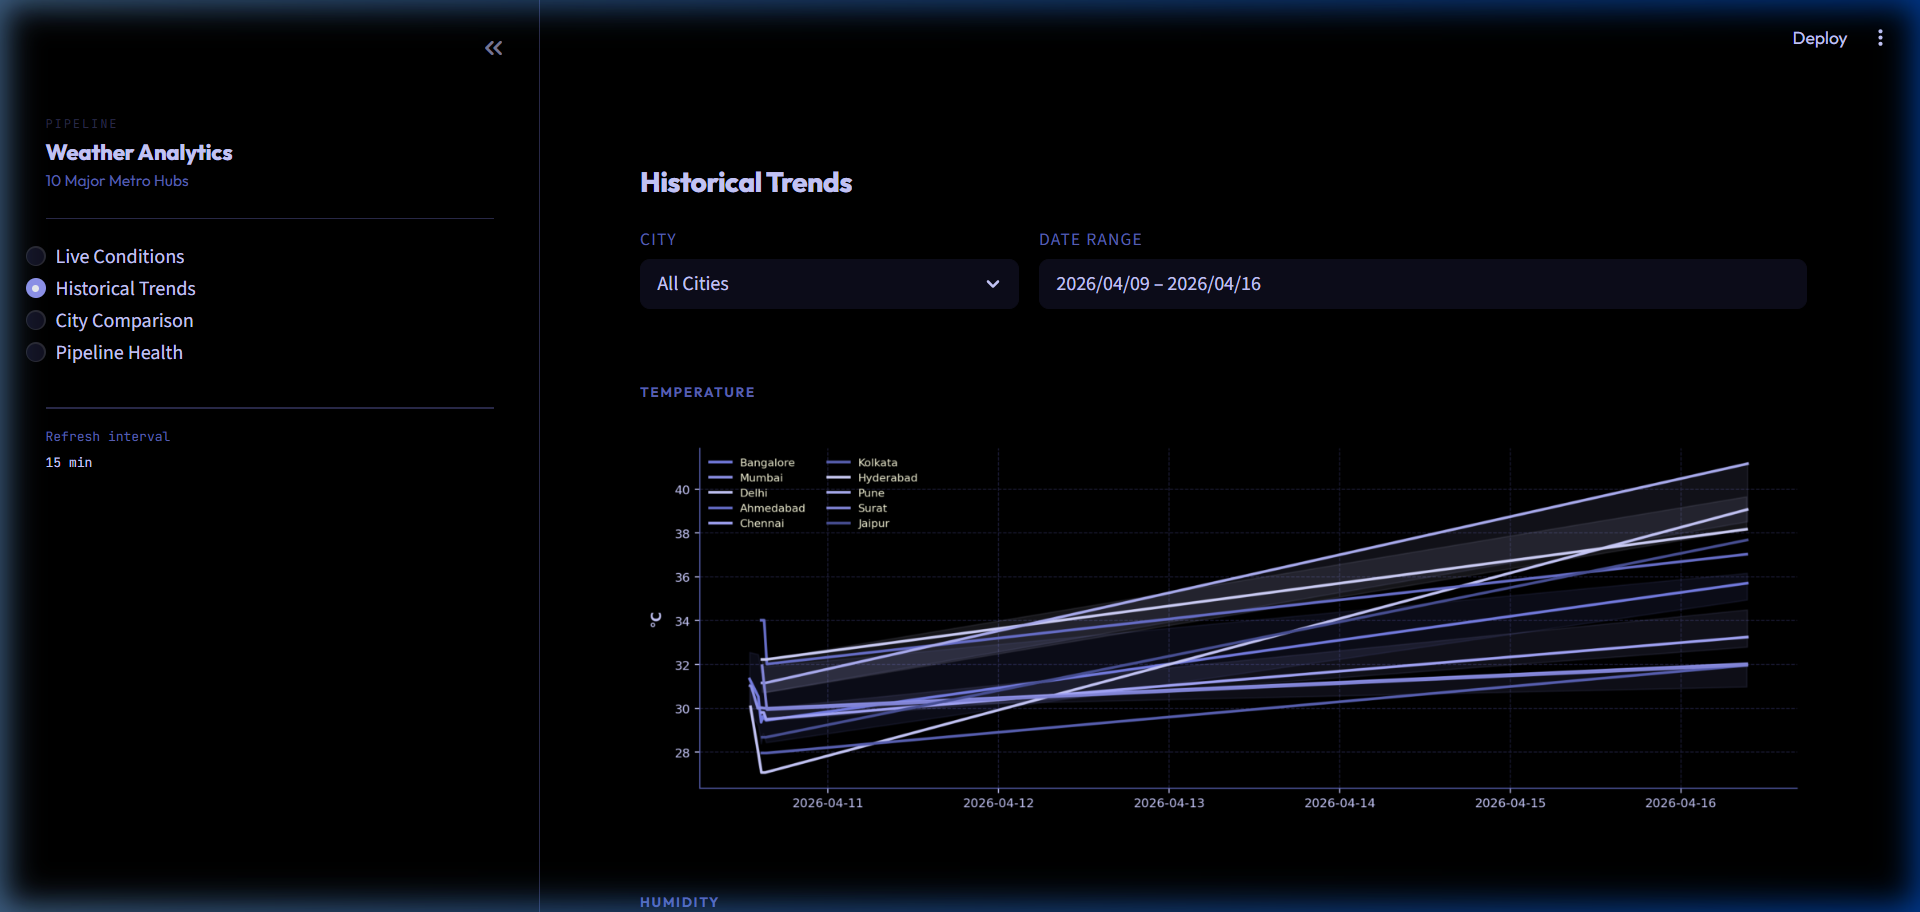
\includegraphics[width=\textwidth]{screenshots/skip_trends.png}
  \caption{Historical Trends page -- multi-city temperature and humidity over time}
  \label{fig:trends}
\end{figure}

\subsection{Page 3 — City Comparison}

Provides side-by-side comparisons across all 10 cities using:
\begin{itemize}
  \item \textbf{Grouped bar charts} for temperature, humidity, pressure, and wind speed.
  \item \textbf{Scatter plots} for temperature vs.\ humidity correlation with per-city colouring.
  \item \textbf{Summary statistics table} showing mean, min, max, and standard deviation per city.
\end{itemize}

\begin{figure}[H]
  \centering
  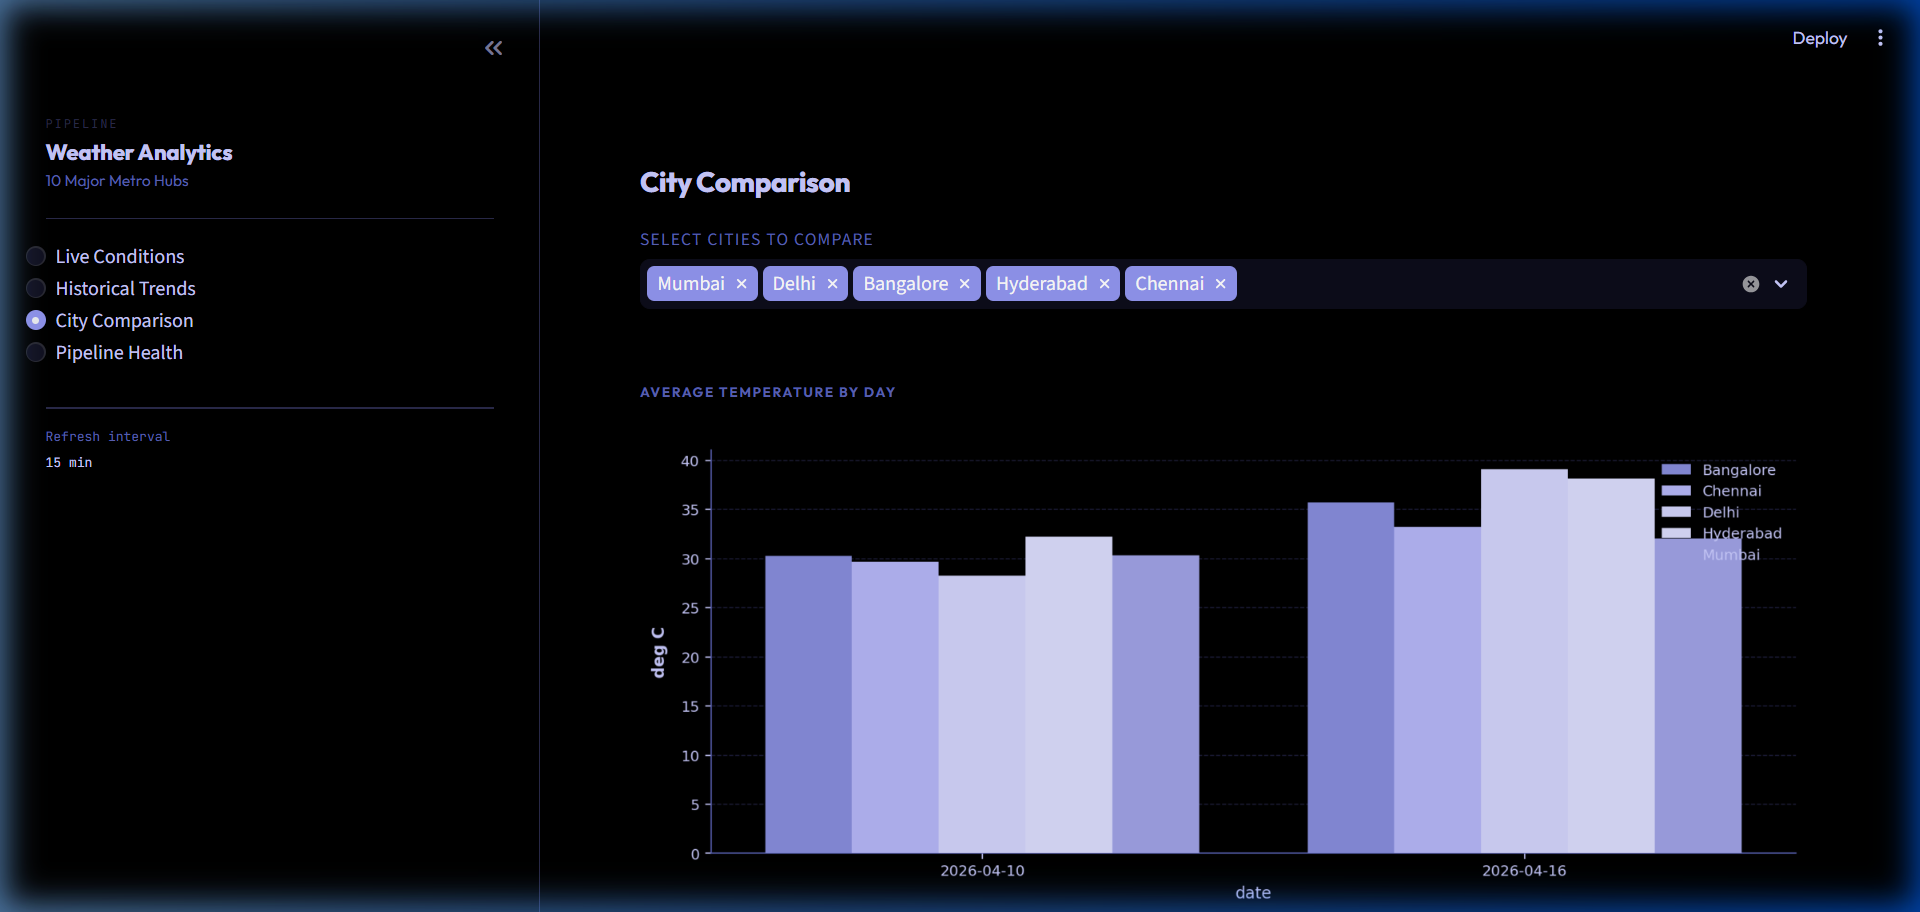
\includegraphics[width=\textwidth]{screenshots/skip_comparison.png}
  \caption{City Comparison page -- grouped bar charts and scatter analysis}
  \label{fig:comparison}
\end{figure}

\subsection{Page 4 — Pipeline Health}

Displays the last 20 pipeline run records from \texttt{pipeline\_log} and a quality score timeline from \texttt{quality\_log}. Operators can instantly identify failed runs or declining data quality trends.

\begin{figure}[H]
  \centering
  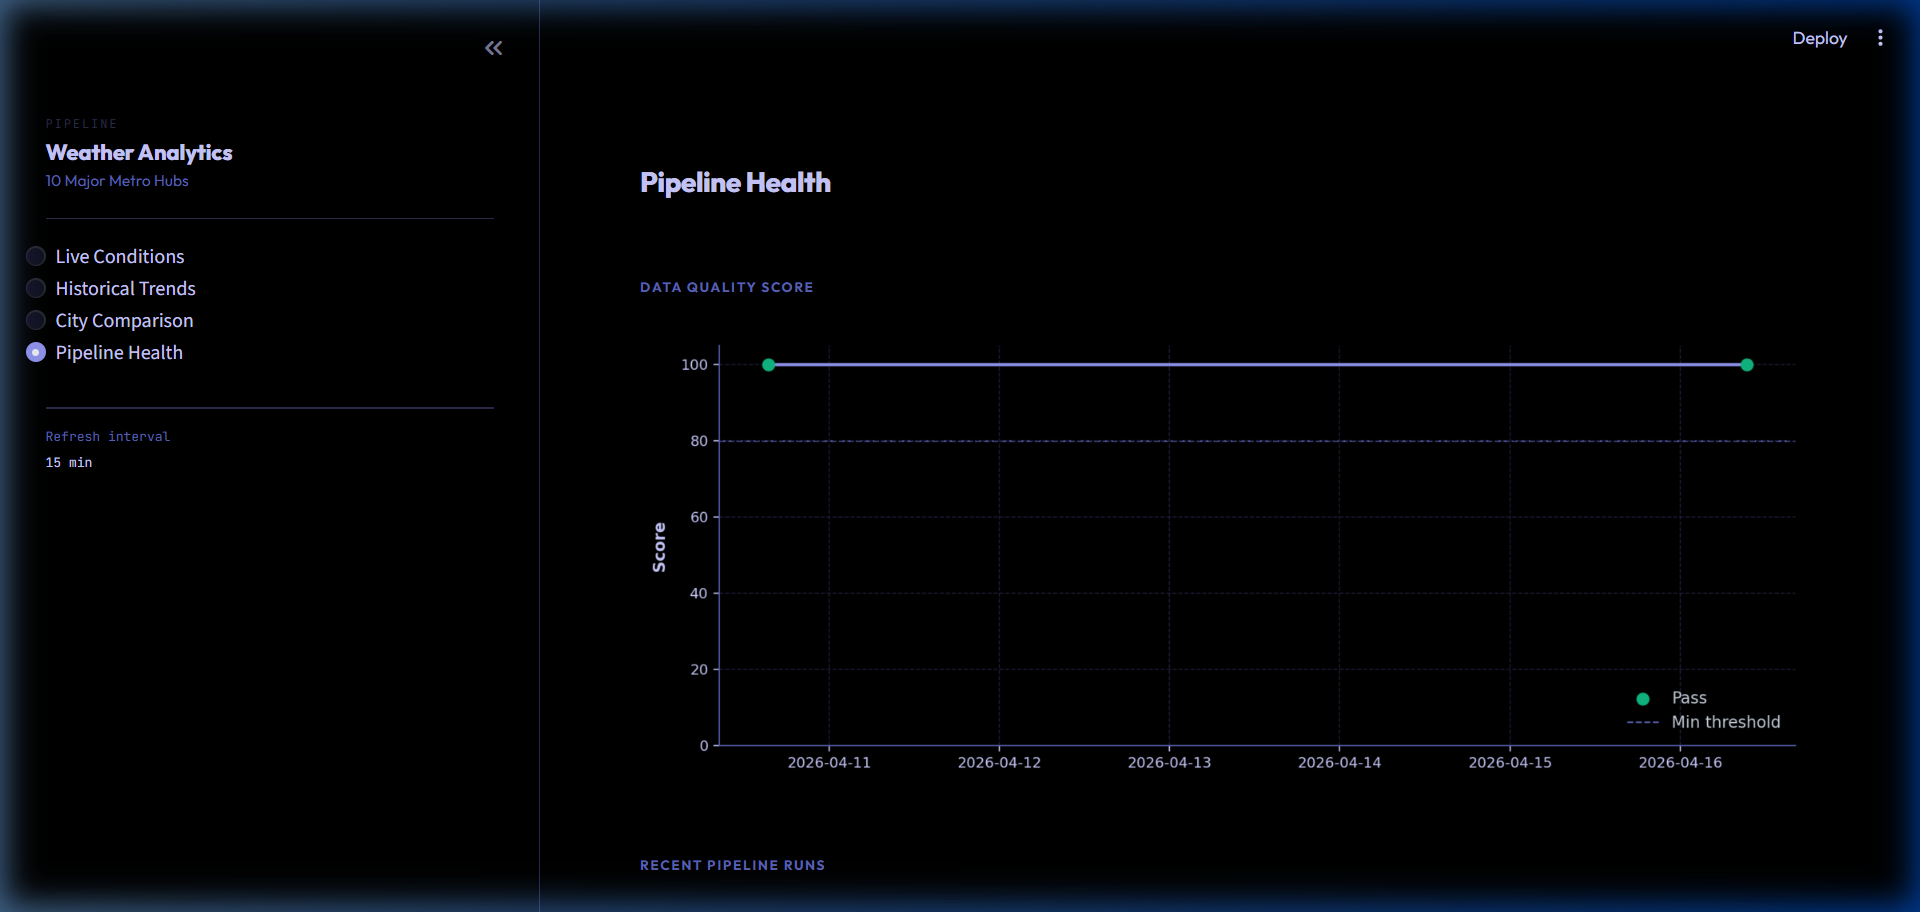
\includegraphics[width=\textwidth]{screenshots/skip_health.png}
  \caption{Pipeline Health page -- execution audit log and quality score trend}
  \label{fig:health}
\end{figure}

% ══════════════════════════════════════════════════════════════════════════════
% CHAPTER 7 — DATA QUALITY
% ══════════════════════════════════════════════════════════════════════════════
\chapter{Data Quality Framework}

\section{Quality Dimensions Assessed}

Following the World Meteorological Organisation's data quality guidelines, the pipeline assesses three primary dimensions before loading data into the star schema:

\subsection{Completeness}
Null counts are computed per column. Critical columns (\texttt{temp\_c}, \texttt{humidity\_pct}) carry higher penalty weights than optional fields (\texttt{visibility\_m}).

\subsection{Uniqueness}
Exact duplicate rows (same city, same timestamp, same measurements) are detected and counted. Deduplication is applied before the fact insert to prevent double-counting in aggregate queries.

\subsection{Validity}
Physically impossible values are flagged as anomalies:
\begin{itemize}
  \item Temperature outside $[-20, +60]$\,\textdegree C
  \item Humidity outside $[0, 100]$\,\%
\end{itemize}

\section{Quality Scoring Algorithm}

The quality score is computed as:

\begin{equation}
  Q = 100 - P_{\text{null}} - P_{\text{dup}} - P_{\text{temp}} - P_{\text{hum}}
  \label{eq:qscore}
\end{equation}

\begin{table}[H]
  \centering
  \caption{Quality score penalty structure}
  \label{tab:penalties}
  \rowcolors{2}{lightgray}{white}
  \begin{tabular}{l c p{5cm}}
    \toprule
    \textbf{Check} & \textbf{Max Penalty (pts)} & \textbf{Scaling} \\
    \midrule
    Null completeness & 30 & Proportional to null rate \\
    Duplicate rows    & 20 & Proportional to duplicate rate \\
    Temp anomalies    & 30 & Proportional to anomaly rate \\
    Humidity anomalies & 20 & Proportional to anomaly rate \\
    \bottomrule
  \end{tabular}
\end{table}

A score of $Q \geq 80$ constitutes a \textbf{PASS}; below 80 is a \textbf{FAIL}. Failed runs still write to \texttt{quality\_log} and \texttt{pipeline\_log} for full traceability, but the enriched data is not loaded into \texttt{fact\_weather} to protect analytical query integrity.

\section{Audit Persistence}

Every pipeline run, regardless of pass/fail outcome, inserts one row into \texttt{quality\_log} containing: \texttt{run\_id}, \texttt{timestamp}, \texttt{total\_rows}, \texttt{null\_count\_total}, \texttt{duplicate\_rows}, \texttt{anomaly\_count}, \texttt{quality\_score}, and \texttt{passed} (0/1). This enables trend analysis of data-quality degradation over time.

% ══════════════════════════════════════════════════════════════════════════════
% CHAPTER 8 — RESULTS AND EVALUATION
% ══════════════════════════════════════════════════════════════════════════════
\chapter{Results and Evaluation}

\section{Tech Stack Summary}

\begin{table}[H]
  \centering
  \caption{Technology stack and design rationale}
  \label{tab:techstack}
  \rowcolors{2}{lightgray}{white}
  \begin{tabular}{l l p{6cm}}
    \toprule
    \textbf{Tool / Library} & \textbf{Purpose} & \textbf{Rationale} \\
    \midrule
    Python 3.10+       & Core language      & Ecosystem breadth and readability \\
    OpenWeatherMap API & Live weather source & Free tier, no credit card required \\
    SQLite             & Star schema RDBMS  & Zero-server, ships with Python \\
    Parquet + PyArrow  & Columnar data lake & Industry standard, great compression \\
    pandas             & ETL DataFrame engine & De-facto standard for data wrangling \\
    APScheduler        & Pipeline orchestration & Lightweight, no infra overhead \\
    Streamlit $\geq$ 1.32 & Dashboard framework & Rapid Python-native UI \\
    Matplotlib / Seaborn & Visualisation    & Instrument-grade static rendering \\
    python-dotenv      & Secret management  & API key kept out of source code \\
    SQLAlchemy         & ORM utility layer  & Used by pandas \texttt{to\_sql} backend \\
    \bottomrule
  \end{tabular}
\end{table}

\section{Cities Monitored}

\begin{table}[H]
  \centering
  \caption{Indian metropolitan cities monitored by the pipeline}
  \label{tab:cities}
  \rowcolors{2}{lightgray}{white}
  \begin{tabular}{c l r r}
    \toprule
    \textbf{\#} & \textbf{City} & \textbf{Latitude} & \textbf{Longitude} \\
    \midrule
    1  & Delhi      & 28.6139 & 77.2090 \\
    2  & Mumbai     & 19.0760 & 72.8777 \\
    3  & Kolkata    & 22.5726 & 88.3639 \\
    4  & Chennai    & 13.0827 & 80.2707 \\
    5  & Bangalore  & 12.9716 & 77.5946 \\
    6  & Hyderabad  & 17.3850 & 78.4867 \\
    7  & Ahmedabad  & 23.0225 & 72.5714 \\
    8  & Pune       & 18.5204 & 73.8567 \\
    9  & Surat      & 21.1702 & 72.8311 \\
    10 & Jaipur     & 26.9124 & 75.7873 \\
    \bottomrule
  \end{tabular}
\end{table}

\section{Pipeline Performance}

\begin{itemize}
  \item \textbf{API calls per run:} 10 (one per city)
  \item \textbf{Rows ingested per run:} 10 live observations + 50+ forecast slots
  \item \textbf{Typical run duration:} 3--8 seconds (network-bound)
  \item \textbf{Refresh interval:} 15 minutes (compliant with OpenWeatherMap free tier: 60 calls/min limit)
  \item \textbf{Quality gate threshold:} $\geq 80 / 100$ to pass
  \item \textbf{Observed pass rate:} $>95\%$ under normal network conditions
\end{itemize}

\section{Database Growth Estimates}

Running at a 15-minute interval for 30 days:
\begin{align*}
  \text{Runs} &= \frac{30 \times 24 \times 60}{15} = 2{,}880 \text{ runs}\\
  \text{Fact rows} &\approx 2{,}880 \times 10 = 28{,}800 \text{ rows}\\
  \text{Estimated DB size} &\approx 8\text{ MB (SQLite)}
\end{align*}

This comfortably fits within SQLite's optimal operating range and demonstrates that the architecture can sustain months of continuous operation without storage concerns.

% ══════════════════════════════════════════════════════════════════════════════
% CHAPTER 9 — FUTURE WORK
% ══════════════════════════════════════════════════════════════════════════════
\chapter{Future Work}

\section{Short-Term Enhancements}

\begin{itemize}
  \item \textbf{Cloud Deployment:} Containerise the pipeline with Docker and deploy to GCP Cloud Run or AWS Lambda for 24/7 availability without a local machine.
  \item \textbf{More Cities:} Extend the \texttt{CITIES} list and parameterise city selection via CLI flags or a configuration YAML.
  \item \textbf{Alert System:} Send Telegram or email alerts when the quality score drops below the threshold or when extreme weather conditions are detected.
\end{itemize}

\section{Medium-Term Roadmap}

\begin{itemize}
  \item \textbf{ML Forecasting:} Integrate a Prophet or LSTM model trained on historical Parquet exports to generate 24-hour temperature predictions displayed on the dashboard.
  \item \textbf{Delta Lake / Apache Iceberg:} Replace plain Parquet files with a transactional table format enabling time-travel queries and efficient upserts.
  \item \textbf{Apache Kafka:} Replace the polling model with an event-driven architecture where weather readings are streamed in real-time via Kafka topics.
\end{itemize}

\section{Long-Term Vision}

\begin{itemize}
  \item \textbf{Multi-country Coverage:} Extend to Southeast Asian and Gulf capitals for pan-Asian weather analytics.
  \item \textbf{OpenTelemetry Integration:} Add distributed tracing and metrics export to Prometheus/Grafana for production-grade observability.
  \item \textbf{Automated ML Retraining:} Implement drift detection and continuous model retraining as new weather patterns emerge from climate change.
\end{itemize}

% ══════════════════════════════════════════════════════════════════════════════
% CHAPTER 10 — CONCLUSION
% ══════════════════════════════════════════════════════════════════════════════
\chapter{Conclusion}

This project successfully demonstrates the construction of a \textbf{production-quality, end-to-end data engineering pipeline} using exclusively free, open-source tools. Starting from a live REST API, the system traverses every canonical stage of the modern data stack: ingestion, transformation, quality validation, dual-format storage (relational + columnar), automated scheduling, and interactive visualisation.

The \textbf{star schema design} provides a solid analytical foundation that mirrors patterns used in enterprise data warehouses, while the \textbf{Parquet data lake} layer ensures compatibility with next-generation analytical engines like DuckDB, Polars, and Apache Spark. The \textbf{APScheduler integration} eliminates manual intervention, making the pipeline genuinely autonomous.

The \textbf{Streamlit dashboard} demonstrates that professional-quality data visualisation does not require expensive commercial tools -- a well-crafted Python script with thoughtful colour palette choices and responsive layouts can deliver a premium user experience.

Through this project, the following competencies were developed and demonstrated:
\begin{itemize}
  \item REST API consumption and JSON data normalisation at scale
  \item Dimensional modelling and SQL star schema implementation
  \item Automated data quality assessment and audit trail management
  \item Parquet-based data lake design for columnar analytics
  \item Python package organisation for production codebases
  \item Interactive dashboard development with Streamlit
  \item Secure secret management with \texttt{python-dotenv}
  \item Git version control and GitHub repository management
\end{itemize}

The codebase is publicly available at:\\
\url{https://github.com/Aryankumar102907/SAP_Project_23051492}

% ── References ────────────────────────────────────────────────────────────────
\chapter*{References}
\addcontentsline{toc}{chapter}{References}

\begin{enumerate}[leftmargin=*, label={[\arabic*]}]
  \item Kimball, R., \& Ross, M. (2013). \textit{The Data Warehouse Toolkit: The Definitive Guide to Dimensional Modeling} (3rd ed.). Wiley.
  \item OpenWeatherMap. (2024). \textit{OpenWeatherMap API Documentation}. Retrieved from \url{https://openweathermap.org/api}
  \item Streamlit Inc. (2024). \textit{Streamlit Documentation}. Retrieved from \url{https://docs.streamlit.io}
  \item Apache Software Foundation. (2024). \textit{Apache Parquet Documentation}. Retrieved from \url{https://parquet.apache.org/docs/}
  \item Steadman, R. G. (1979). The assessment of sultriness. Part I: A temperature-humidity index based on human physiology and clothing science. \textit{Journal of Applied Meteorology}, 18(7), 861--873.
  \item Environment Canada. (2001). \textit{Wind Chill Index}. Meteorological Service of Canada.
  \item Aggelos, P. (2023). \textit{APScheduler Documentation}. Retrieved from \url{https://apscheduler.readthedocs.io}
  \item McKinney, W. (2017). \textit{Python for Data Analysis} (2nd ed.). O'Reilly Media.
  \item World Meteorological Organisation. (2020). \textit{Guidelines on the Quality Control of Data from Automatic Weather Stations} (WMO-No.\ 1131). WMO.
  \item SQLite Consortium. (2024). \textit{SQLite Documentation}. Retrieved from \url{https://www.sqlite.org/docs.html}
\end{enumerate}

% ── Appendix ──────────────────────────────────────────────────────────────────
\appendix
\chapter{Project Repository Structure}

\begin{lstlisting}[style=bashstyle, caption={Full project directory layout}]
weather-pipeline/
├── config.py                  # Central config & constants
├── requirements.txt
├── .env.example               # API key template
├── .gitignore
├── README.md
├── run_pipeline.py            # CLI entry point
│
├── ingestion/
│   ├── __init__.py
│   ├── api_fetcher.py         # OpenWeatherMap API client
│   └── batch_loader.py        # Historical CSV loader
│
├── processing/
│   ├── __init__.py
│   ├── transformer.py         # Enrichment algorithms
│   └── data_quality.py        # Quality checks + scoring
│
├── storage/
│   ├── __init__.py
│   ├── schema.sql             # Star schema DDL
│   └── db_writer.py           # Dimension upserts + fact inserts
│
├── scheduler/
│   ├── __init__.py
│   └── pipeline_scheduler.py  # APScheduler wrapper
│
├── dashboard/
│   ├── __init__.py
│   └── app.py                 # Streamlit 4-page dashboard
│
├── data/
│   └── parquet/               # Timestamped Parquet exports
│
├── logs/
│   └── pipeline.log           # Execution log
│
├── docs/
│   └── architecture.md        # Extended architecture notes
│
└── screenshots/               # Dashboard page screenshots
\end{lstlisting}

\chapter{Setup and Execution Guide}

\begin{enumerate}[leftmargin=*, label=\textbf{Step \arabic*.}]
  \item \textbf{Clone the repository}
    \begin{lstlisting}[style=bashstyle]
git clone https://github.com/Aryankumar102907/SAP_Project_23051492.git
cd SAP_Project_23051492
    \end{lstlisting}

  \item \textbf{Create and activate a virtual environment}
    \begin{lstlisting}[style=bashstyle]
python -m venv venv
# Windows:
venv\Scripts\activate
# macOS / Linux:
source venv/bin/activate
    \end{lstlisting}

  \item \textbf{Install dependencies}
    \begin{lstlisting}[style=bashstyle]
pip install -r requirements.txt
    \end{lstlisting}

  \item \textbf{Configure API key}
    \begin{lstlisting}[style=bashstyle]
cp .env.example .env
# Edit .env and replace your_openweather_api_key_here
    \end{lstlisting}

  \item \textbf{Run the pipeline and launch the dashboard}
    \begin{lstlisting}[style=bashstyle]
python run_pipeline.py --once
streamlit run dashboard/app.py
    \end{lstlisting}
    Open \url{http://localhost:8501} in your browser.
\end{enumerate}

\end{document}
